%!TEX root = ../thesis.tex

\chapter{Analyse} % (fold)
\label{cha:analyse}

\todo[inline]{Inhalt: wass gibt es, was muss neu gemacht werden}
\todo[inline]{Begriff soziales Netzwerk anpassen}

Um sich eine Vorstellung davon zu machen, wie ein System auszusehen hat und welche Komponenten dazu nötig sind um zwei oder mehrere sozialen Netzwerke zu verbinden, soll hierzu ein kleines Ablaufbeispiel konstruiert werden.Das vollständige Ablaufdiagramm befindet sich im Anhang \ref{sec:anforderungsanalyse_ablaufdiagramm}. 

\section{Neuen Beitrag verfassen} % (fold)
\label{sec:neuen_beitrag_verfassen}

% section neuen_beitrag_verfassen (end)

Alles beginnt damit, dass zum Beispiel ein Student im sozialen Netzwerk A, im Forum zur Veranstaltung Telekooperation 1, eine Frage zur aktuellen Übung stellen will. Er geht zuerst in den passenden Thread und beginnt einen neuen Beitrag zu schreiben. Sobald er fertig ist, klickt er auf \enquote{Absenden} und sein Beitrag wird in der Datenbank des sozialen Netzwerkes A gespeichert und als neuer Eintrag im Thread angezeigt (siehe Abbildung \ref{fig:beutzer_erstellt_beitrag_a}).

\medskip

\begin{figure}[ht]
     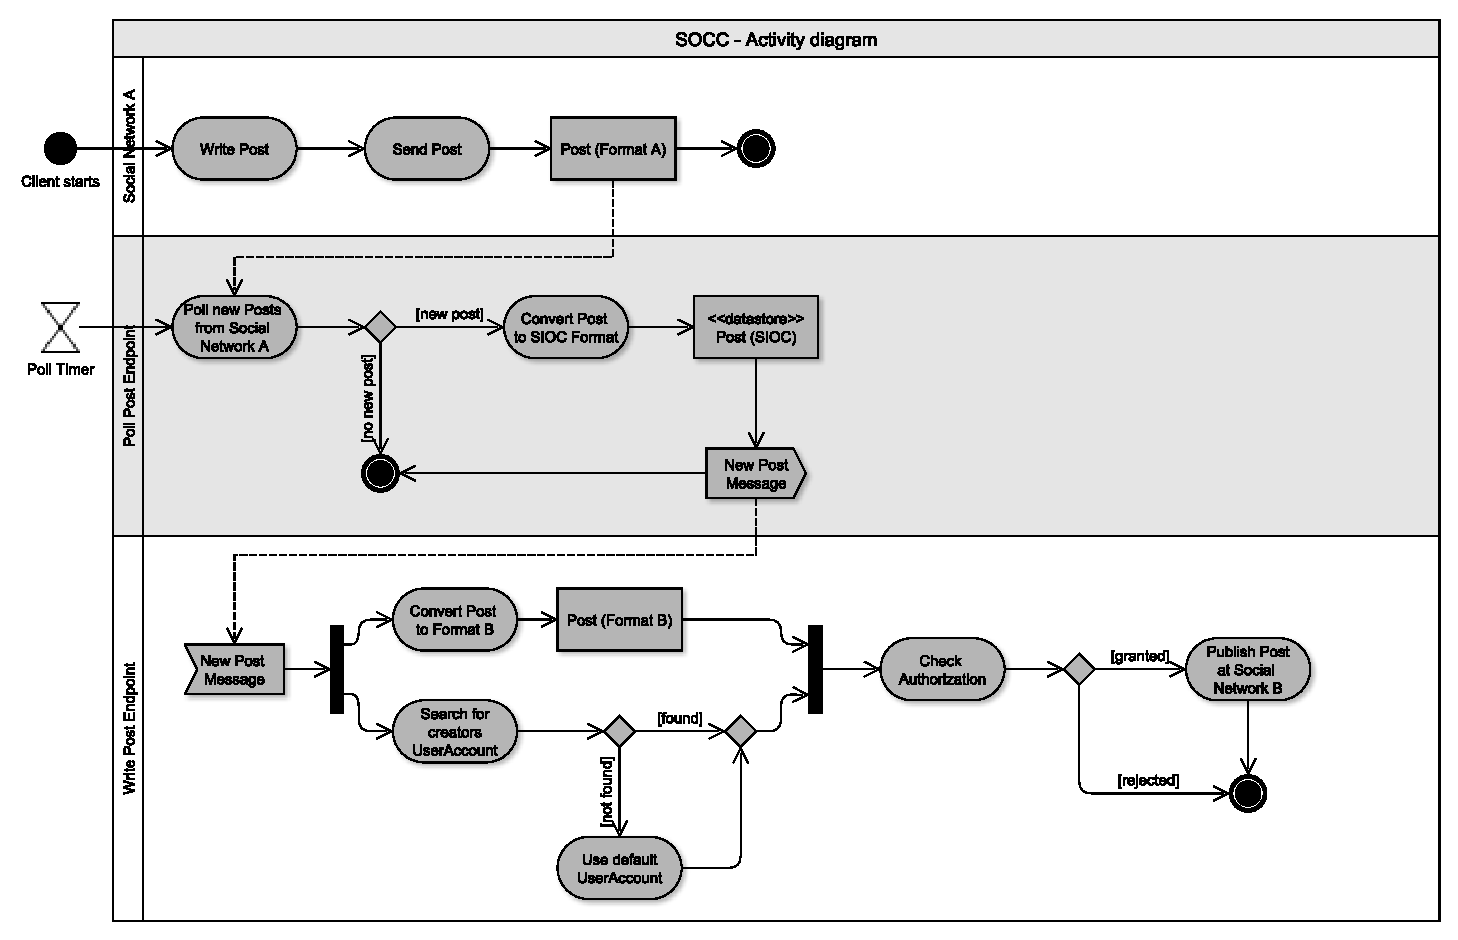
\includegraphics[
        width=\textwidth,
        keepaspectratio=true,
        clip=true,
        trim= 0 338 0 27
    ]{assets/images/activitydiagram_post_as_user_check_authorization.pdf}
    \caption{Benutzer erstellt einen Beitrag im sozialen Netzwerk A.}
    \label{fig:beutzer_erstellt_beitrag_a}
\end{figure}

\section{Beiträge von sozialen Netzwerk A lesen} % (fold)
\label{sec:beiträge_von_solzialen_netzwerk_a_lesen}


Um diese Beitrag in das soziale Netzwerk B transferieren zu können, müssen zuerst die Daten über eine öffentliche Schnittstelle vom Server des sozialen Netzwerks A heruntergeladen werden. Da in der Regel nicht automatisch bekannt ist, wann ein neuer Beitrag vorhanden ist, müssen die Server in zeitlichen Abständen abgefragt (polling genannt) und die zurückgelieferten Daten nach neuen Beiträgen durchsucht werden. Sind ein oder mehrere neue Beiträge gefunden worden, können diese nicht direkt an das soziale Netzwerk B geschickt werden, da sich diese in der Regel im verwendeten Datenformat unterscheiden. Diese müssen zuvor konvertiert werden.

\medskip

Die einfachste Möglichkeit wäre nun die Daten von Format A nach Format B zu konvertieren. Bei zwei Formaten ist dies noch sehr einfach. Es müsste lediglich ein Konverter von Format A nach Format B und einer in die umgekehrte Richtung implementiert werden. Für den Fall, dass nun ein weiteres Netzwerk C unterstützt werden soll, würde ich die Anzahl an nötigen Konvertern auf Sechs erhöhen, wie Tabelle \ref{tbl:anzahl_konvertern_bei_drei_netzwerken} zeigt. 

 \medskip

% \begin{table}[ht]
%     \centering
%     \begin{tabular}{cc}
%         A $ \Rightarrow $ B & A $ \Rightarrow $ C \\
%         B $ \Rightarrow $ A & B $ \Rightarrow $ C \\
%         C $ \Rightarrow $ A & C $ \Rightarrow $ B \\
%     \end{tabular}

    
%     \caption{Konverter bei Drei sozialen Netzwerken}
%     \label{tbl:anzahl_konvertern_bei_drei_netzwerken}
% \end{table}

\begin{table}[ht]
    \centering
    \caption{Anzahl Konverter bei drei sozialen Netzwerken}
    
    \begin{tabular}{c|c|c|c|c}
        % Zeile 1
        \multicolumn{2}{c|}{\multirow{2}{*}{}} & 
        \multicolumn{3}{|c}{\textbf{Nach}}   \\ 
        \cline{3-5} 

        % Zeile 2
        \multicolumn{2}{c|}{} & 
        \textbf{Netzwerk A} & 
        \textbf{Netzwerk B} & 
        \textbf{Netzwerk C} \\ 
        \hline

        % Zeile 3
        \multirow{3}{*}{Von} & 
        \textbf{Netzwerk A} & 
        -&            
        $ \times $ &            
        $ \times $ \\ 
        \cline{2-5} 

        % Zeile 4
        & 
        \textbf{Netzwerk B} &            
        $ \times $ &            
        -&            
        $ \times $ \\ 
        \cline{2-5} 
         
        % Zeile 5
        & 
        \textbf{Netzwerk C} &            
        $ \times $ &            
        $ \times $ &            
        -\\
    \end{tabular}
    \label{tbl:anzahl_konvertern_bei_drei_netzwerken}
\end{table}

Nimmt man an $n_{sn}$ sei eine beliebige Anzahl sozialer Netzwerke, entspricht die Anzahl der notwendiger Konverter $ n_{k1}= n_{sn}*(n_{sn}-1) $, da für jedes Netzwerk ein Konverter in alle anderen Netzwerke erzeugt werden muss. Sollen nur Zwei oder Drei Netzwerke unterstützt werden ist der Aufwand noch sehr überschaubar, bei mehr kann dies aber sehr Aufwendig werden. 

\medskip

Eine elegantere Methode, welche die Anzahl zu implementierender Konverter in Grenzen halten kann, wäre die Einführung eines Zwischenformates. Geht man davon aus, dass die Daten aller Netzwerke nur in dieses Zwischenformat geschrieben und aus diesem gelesen werden müssen, würde sich der Aufwand auf maximal Zwei Konverter pro neuem Netzwerk reduzieren. Für eine beliebige Anzahl Netzwerke wären also $ n_{k2} = n_{sn} * 2 $ Konverter nötig. Nachteile hätte dieser Ansatz nur für $ n_{sn}=2 $ und $ n_{sn}=3$ , da in diesen Fällen mehr beziehungsweise gleich viele Konverter gegenüber der ersten Methode erforderlich wären. Erhöht man die Anzahl Netzwerke jedoch nur geringfügig, sinkt die Menge an Konvertern sichtbar. Für $ n_{sn} = 4 $ wären es $ n_{k2} = 8 $ statt $ n_{k1} = 12 $ und für $ n_{sn} = 5 $ ergibt sich $ n_{k2} = 10 $ statt $ n_{k1} = 20 $ Konvertern. Gleichzeitig können so syntaktische Unterschiede in den einzelnen Formaten angeglichen werden, was sie leichter handhabbar macht. Abbildung \ref{fig:lesen_von_beitrag_und_convertieren} verdeutlicht den Ablauf unter Verwendung des eben beschriebenen Zwischenformats.

\medskip

\begin{figure}[ht]
     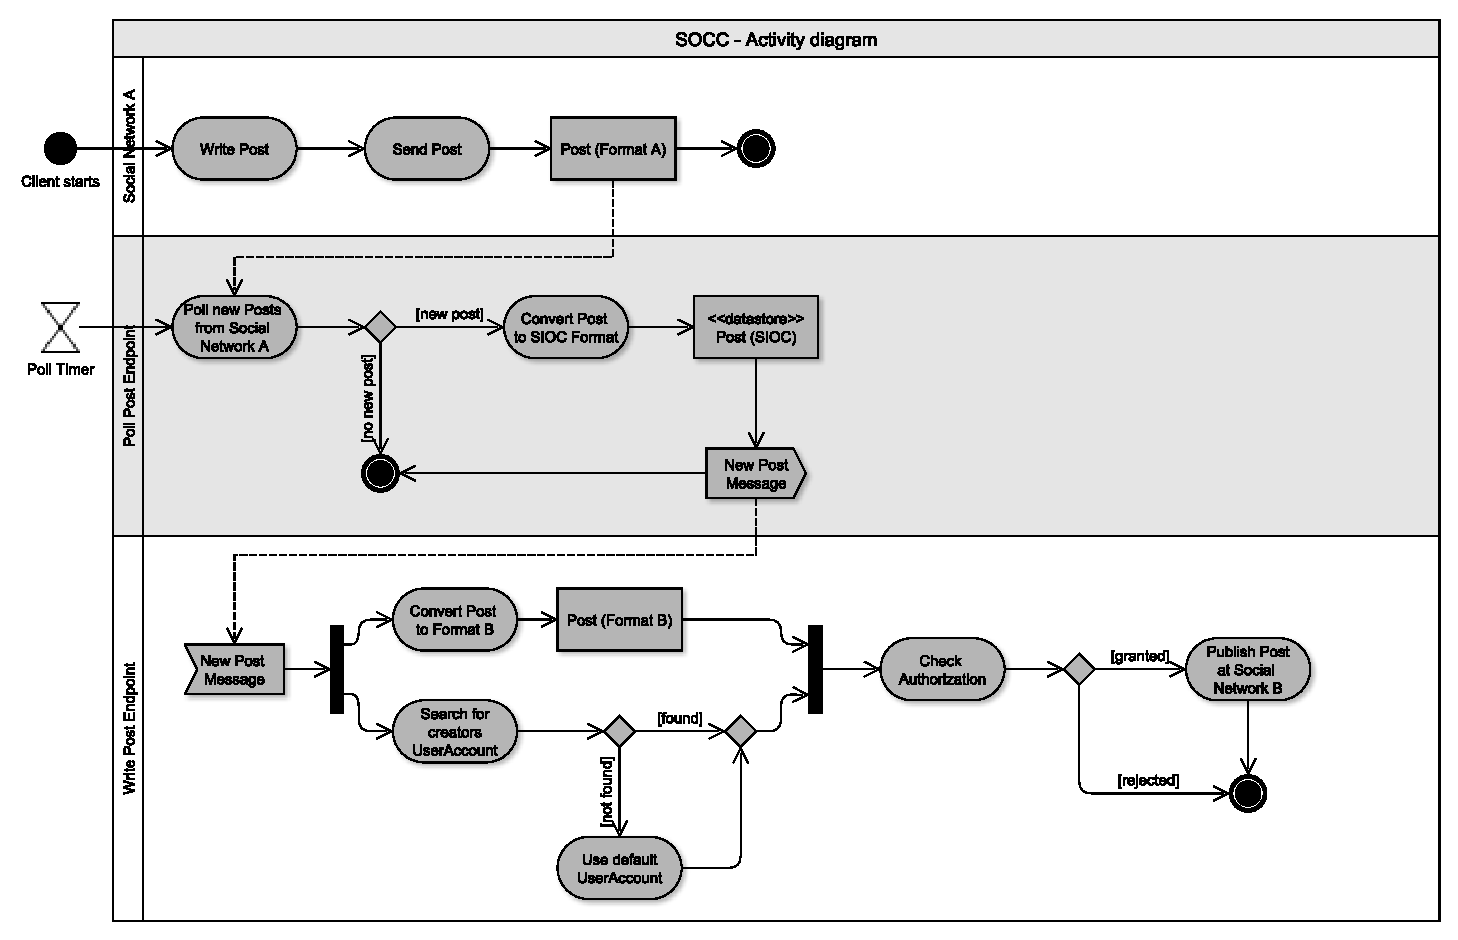
\includegraphics[
        width=\textwidth,
        keepaspectratio=true,
        clip=true,
        trim= 0 193 0 113
    ]{assets/images/activitydiagram_post_as_user_check_authorization.pdf}
    \caption{
        Lesen des erstellten Beitrags und konvertieren in das Zwischenformat.
    }
    \label{fig:lesen_von_beitrag_und_convertieren}
\end{figure}

Liegen nun alle Daten in diesem Zwischenformat vor, könnten diese an einer Datenbank gespeichert werden. Diese Datenbank macht es möglich auf einfache Art und Weise auf die gespeicherten Daten von außerhalb zu zugreifen und diverse Abfragen ausführen zu können. Dies könnte zum Beispiel sein, in den Daten nach inhaltlich gleichen oder ähnlichen Beiträgen zu suchen oder passende externe Materialien aus Vorlesungen zu einen Thema vorzuschlagen. Die Möglichkeiten sind hier vielfältig. 

\medskip

Da ein Teil dieser Arbeit darin besteht Beiträge zwischen zwei oder mehr sozialen Netzwerken zu synchronisieren, muss das Eintreffen neuer Beiträge an die einzelnen Komponenten mitgeteilt werden. Da es unmöglich ist diesen Zeitpunkt vorher zu sagen ist der beste Weg einen ereignisorientierten Ansatz zu wählen. Hierbei wird beim lesen eines neuen Beitrags eine Ereignisnachricht erzeugt, welche die interessierten Komponenten über das Eintreffen informiert. So wird eine zeitliche Entkopplung von Lesen und Schreiben möglich, gleichzeitig können sich einzelnen Komponenten an diesen Nachrichtenstrom an- oder abhängen ohne Andere zu stören. Dies erhöht die Flexibilität des Systems.

% section beiträge_von_solzialen_netzwerk_a_lesen (end)

\section{Beitrag in soziales Netzwerk B schreiben} % (fold)
\label{sec:beitrag_in_soziales_netzwerk_b_schreiben}

Hat sich eine Komponenten und empfängt eine Ereignisnachricht von einen neuen Beitrag, wird ähnlich Verfahren wie schon beim Lesen, nur umgekehrt (Siehe Abbildung \ref{fig:konvertieren_formatb_und_schreiben} links, oberer Ablauf). Der neue Beitrag wird vor den schreiben in das soziale Netzwerk B aus dem Zwischenformat in der Zielformat B konvertiert. Alle dazu nötigen Information können direkt aus der Ereignisnachricht oder zusätzlich aus der oben genannten Datenbank geholt werden. 

\medskip

Wünschenswert wäre es hierbei, wenn es so aussehen würde der Beitrag nicht vom hier entwickelten System, sondern von Autor des ursprünglichen Beitrags geschrieben worden. Hierzu es unerlässlich auf das Konto des Autor im entsprechenden Netzwerk zugreifen zu können, da im allgemeinen der Schreiben stellvertretend für dritte Personen nicht möglich ist. Hierzu muss zunächst für den betreffenden Autor das Konto für das soziale Netzwerk B herausgesucht werden (Siehe Abbildung \ref{fig:konvertieren_formatb_und_schreiben} links, unterer Ablauf). Wurde ein passendes Konto gefunden, wird der konvertierte Beitrag über diesen geschrieben. Sollten kein Passender gefunden werden, müsste dies über ein vorher definiertes Konto geschehen. Dabei sollte aber auf den ursprünglichen Autor beziehungsweise Beitrag in irgendeiner Form hingewiesen werden. Dies kann zum Beispiel durch anbringen eines Links an den  Text des Beitrags erfolgen. 

\medskip

\begin{figure}[ht]
     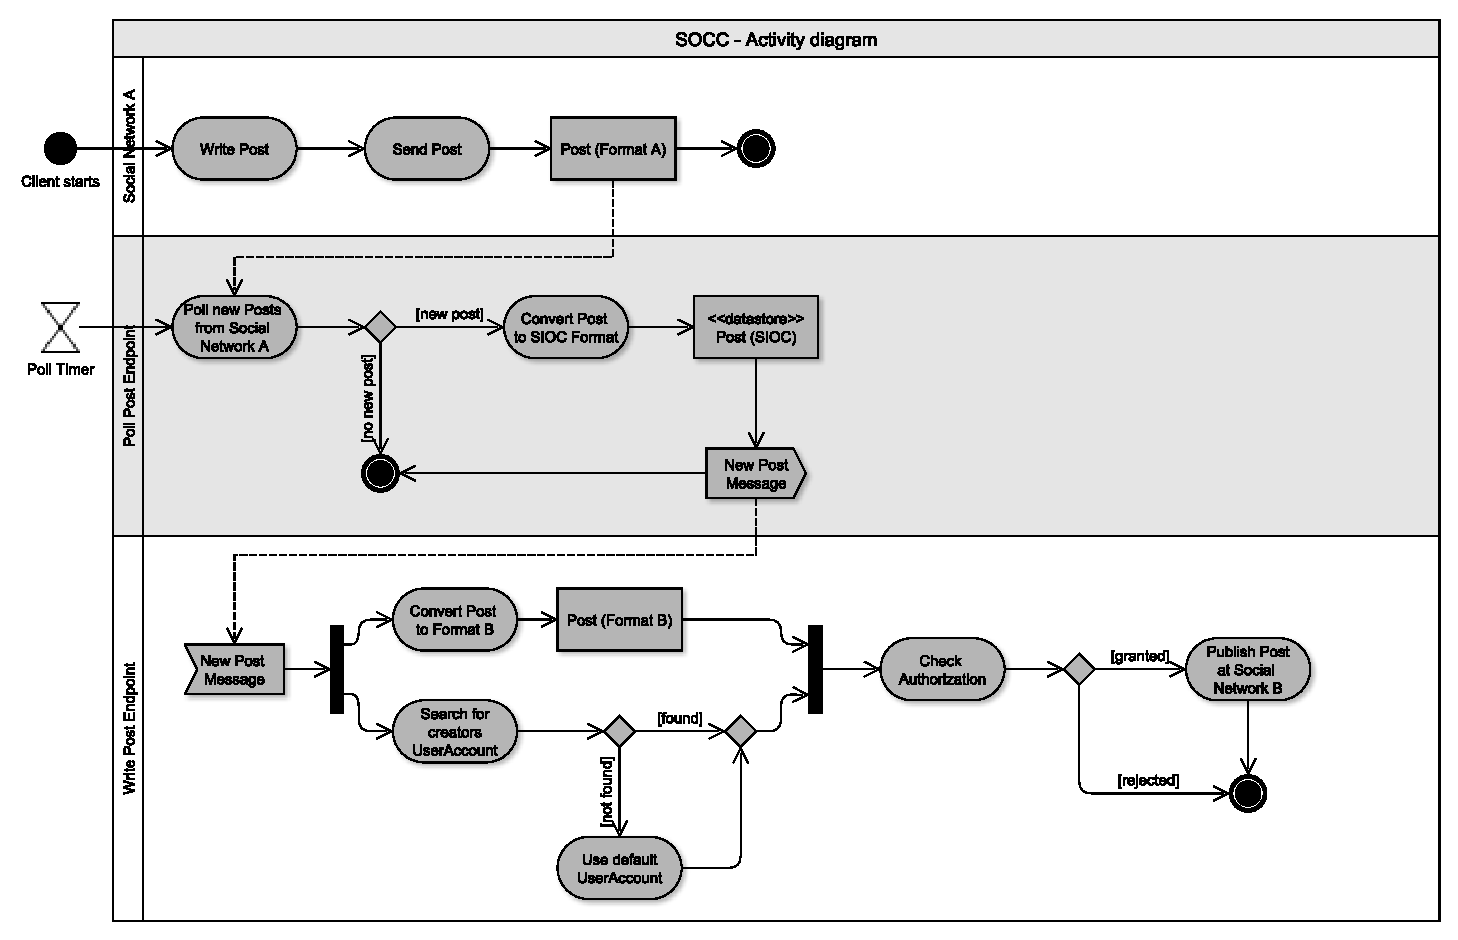
\includegraphics[
        width=\textwidth,
        keepaspectratio=true,
        clip=true,
        trim= 0 0 0 257
    ]{assets/images/activitydiagram_post_as_user_check_authorization.pdf}
    \caption{
        Konvertierten des Beitrags in das Format B und schreiben in das soziale Netzwerk B
    }
    \label{fig:konvertieren_formatb_und_schreiben}
\end{figure}

Gleichzeitig mit den Sammeln von Daten kommt immer auch das Thema zum Schutz der Privatsphäre auf. Wie soll damit umgegangen werden, wen ein Benutzer nicht möchte dass seine Beiträge gesammelt werden oder automatisch weiter geleiten werden sollen? Hierzu wäre es sinnvoll die eben beschriebenen Abläufe so zu erweitern, dass der Benutzer festlegen kann bestimme Quellen oder einzelne Teile für das automatische Lesen und Schreiben zu blockieren, wie es von Uldis Bojars et al. in \cite{Bojars2011} vorgeschlagen wird. Dies könnte durch eine Access Control List (ACL) realisiert werden. Hier könnte der Benutzer Lese und Schreibrechte für einzelne Bereiche festlegen, welche dann das System benutzt um einzelne Abläufe auszuführen oder abzubrechen.

% section beitrag_an_soziales_netzwerk_b_weiterleiten (end)

\section{Identifizierung der Komponenten} % (fold)
\label{sec:identifizierung_der_komponenten}

Anhand dieses kurzen Ablaufbeispiels können wir nun einige Komponenten ablesen die das System unbedingt beinhalten muss und welche ergänzend dazu Wünschenswert wären:

\begin{itemize} 
    \item Eine Komponente muss Daten von einen sozialen Netzwerk in das System einlesen und diese in ein geeignetes Zwischenformat konvertieren können.
    \item Eine weitere Komponente nimmt Beiträte im Zwischenformat entgegen, konvertiert diese in das Format des entsprechenden Netzwerkes und schreibt diese dorthin.
    \item Um stellvertretend für einen Benutzer schreiben zu können muss es möglich sein nach Konto eines Benutzer in einem Netzwerk suchen zu können.
    \item Um die Privatsphäre der Benutzer zu wahren, wäre eine ACL Mechanismus sinnvoll.
\end{itemize}   

% section identifizierung_der_komponenten (end)

% chapter analyse (end)